\begin{figure}

  \centering

  \begin{subfigure}[t]{0.49\textwidth}
    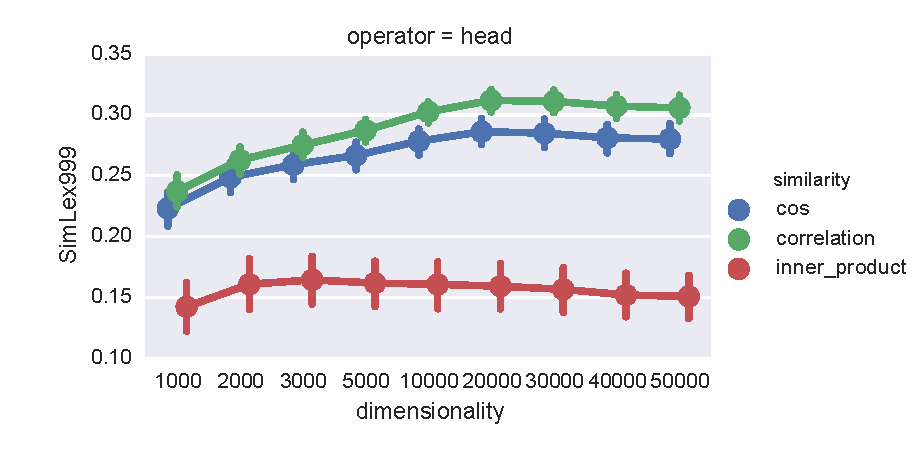
\includegraphics[width=\textwidth]{supplement/figures/SimLex999-interaction-similarity}
    \caption{similarity}
    \label{fig:SimLex999-interaction-similarity}
  \end{subfigure}
  \begin{subfigure}[t]{0.49\textwidth}
    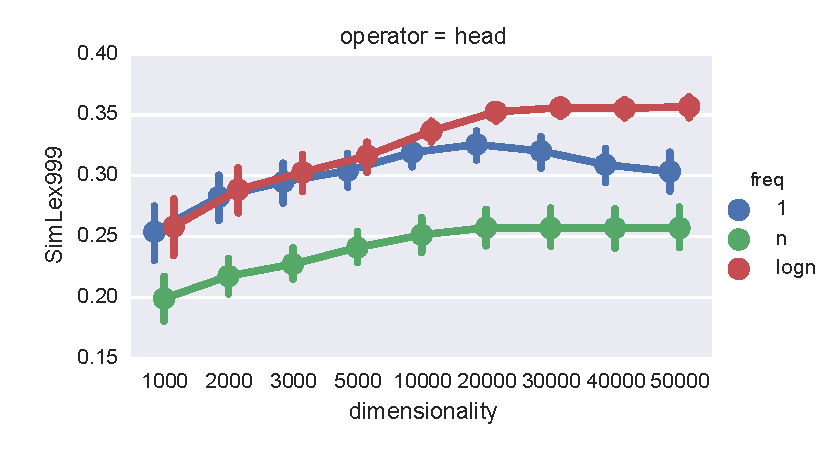
\includegraphics[width=\textwidth]{supplement/figures/SimLex999-interaction-freq}
    \caption{\texttt{freq}}
    \label{fig:SimLex999-interaction-freq}
  \end{subfigure}

  \begin{subfigure}[t]{0.49\textwidth}
    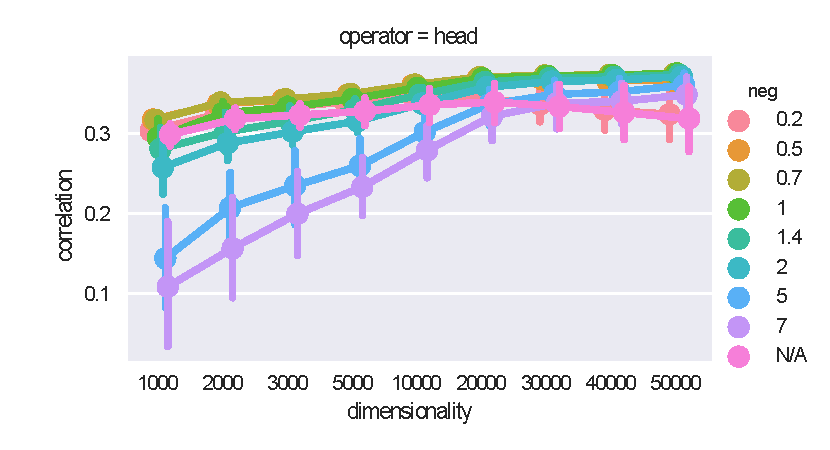
\includegraphics[width=\textwidth]{supplement/figures/SimLex999-interaction-neg}
    \caption{\texttt{neg}}
    \label{fig:SimLex999-interaction-neg}
  \end{subfigure}
  \begin{subfigure}[t]{0.49\textwidth}
    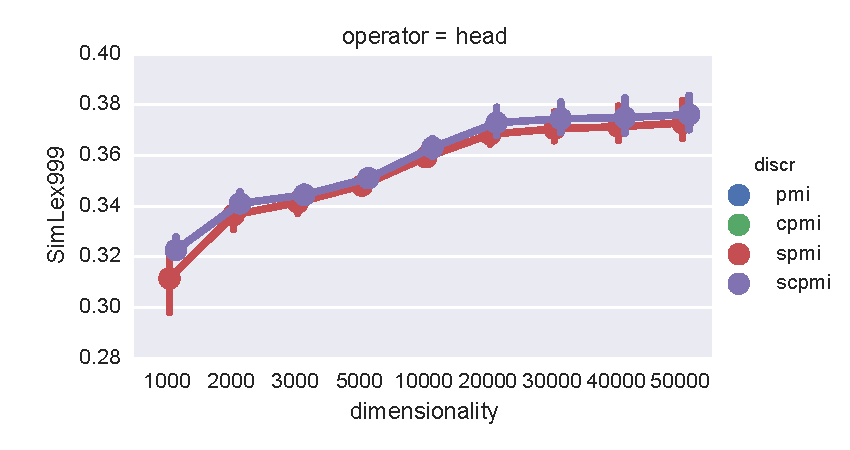
\includegraphics[width=\textwidth]{supplement/figures/SimLex999-interaction-discr}
    \caption{\texttt{discr}}
    \label{fig:SimLex999-interaction-discr}
  \end{subfigure}

  \begin{subfigure}[t]{0.49\textwidth}
    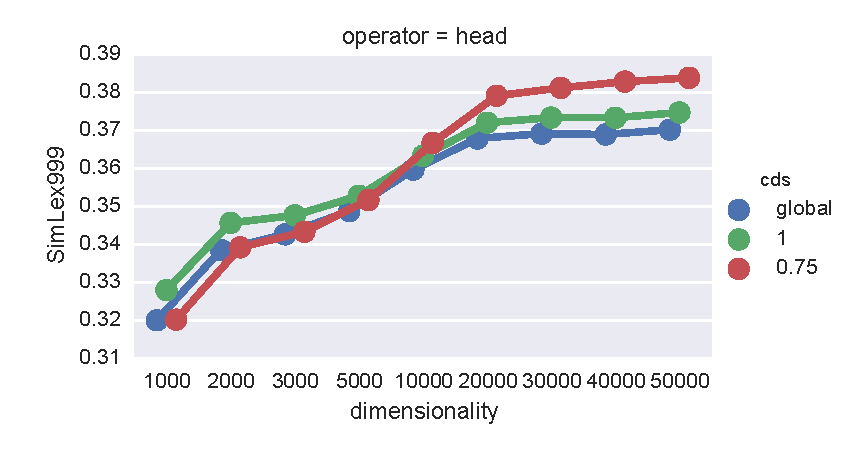
\includegraphics[width=\textwidth]{supplement/figures/SimLex999-interaction-cds}
    \caption{\texttt{cds}}
    \label{fig:SimLex999-interaction-cds}
  \end{subfigure}

  \caption{SimLex-999 parameter interaction. Parameters are shown in the order of their influence.}
  \label{fig:SimLex999-interaction}
\end{figure}

%%% Local Variables:
%%% mode: latex
%%% TeX-master: "../thesis"
%%% End:
